% Final deck: Modules 1-5 in order.
% Build with pdflatex from inside this folder (run it twice for the frame count).
% Each module's frames live in moduleN/moduleN_frames.tex; its figures are in moduleN/figs/.
\documentclass[aspectratio=169,10pt]{beamer}
\usepackage{graphicx,booktabs,amssymb}
\usepackage{tikz}
\usetikzlibrary{arrows.meta,positioning}
\usepackage{multimedia}   % needed by Module 4 if the optional video frame is enabled

\graphicspath{{module1/}{module2/}{module3/}{module4/}{module5/}}

\usetheme{default}
\setbeamertemplate{navigation symbols}{}
\definecolor{deckInk}{HTML}{1F2933}
\definecolor{deckAccent}{HTML}{7B2D8E}
\setbeamercolor{frametitle}{fg=deckInk}
\setbeamercolor{framesubtitle}{fg=deckInk!60}
\setbeamercolor{structure}{fg=deckAccent}
\setbeamerfont{frametitle}{series=\bfseries,size=\large}
\setbeamerfont{framesubtitle}{size=\scriptsize}
\setbeamertemplate{frametitle}{%
  \vspace*{4pt}\insertframetitle\par
  {\usebeamerfont{framesubtitle}\usebeamercolor[fg]{framesubtitle}\insertframesubtitle\par}
  \vskip3pt{\color{deckAccent}\hrule height 0.6pt}\vskip-4pt}
\setbeamertemplate{footline}{\hfill{\scriptsize\color{deckInk!50}\insertframenumber}\hspace*{10pt}\vspace*{6pt}}
\setbeamersize{text margin left=18pt,text margin right=18pt}

\begin{document}

% ---- Title ----
\begin{frame}[plain]
\centering\vspace{10pt}
{\color{deckInk}\Large\bfseries Physics-Informed Neural Networks for Parameter Estimation\\and Hidden-State Recovery in an SEIRD Epidemic Model\\with Time-Varying Transmission\par}
\vspace{4pt}
{\color{deckAccent}\hrule height 0.6pt}
\vspace{6pt}
{\color{deckInk!70}\normalsize The 2014 West African Ebola Outbreak (Sierra Leone)\par}
\vspace{12pt}
{\small\color{deckInk}
Vismay Shanbhag \quad Tanishk Tasgaonkar \quad Lakshya Satya\\
Saatwik Tiwari \quad Nitin Sureshkumar\par}
\vspace{6pt}
{\footnotesize\color{deckInk!60}Group Project: Mathematical Modelling \quad\textbullet\quad October 2026\par}
\end{frame}

% ---- Module 1: motivation, model, published models, phase plane ----
% ======================================================================
% Module 1: motivation, SEIRD model, published models, phase plane
% Four frames, no title slide: \input this file into the main deck.
%
% Needs in the main preamble:  \usepackage{graphicx,booktabs,amssymb,tikz}
%                              \usetikzlibrary{arrows.meta,positioning}
% Figures are in figs/ next to this file. If this file sits in a folder
% (e.g. module1/), add \graphicspath{{module1/}} to the main preamble.
% All numbers are from report/main.tex (final Colab run).
% ======================================================================

% Shared deck colours (same values as Module 5)
\definecolor{mvPINN}{HTML}{7B2D8E}
\definecolor{mvInk}{HTML}{1F2933}
\definecolor{mvMuted}{HTML}{5F6B7A}
\definecolor{mvSoft}{HTML}{F3EDF6}
\definecolor{mvRule}{HTML}{C9B6D3}

\providecommand{\mvTakeaway}[1]{%
  \par\vspace{3pt}\noindent
  \fcolorbox{mvRule}{mvSoft}{\parbox{\dimexpr\linewidth-2\fboxsep-2\fboxrule\relax}{\footnotesize\color{mvInk}#1}}}

% ----------------------------------------------------------------------
\begin{frame}{Why transmission must change over time}
\framesubtitle{Module 1 \textbullet\ Ebola in Sierra Leone, 2014--15 \textbullet\ an SEIRD model with a time-varying transmission rate $\beta(t)$}
\vspace{-2pt}
\begin{columns}[T,onlytextwidth]
\column{0.52\textwidth}
  \footnotesize\raggedright
  \textbf{\color{mvPINN}The problem}
  \begin{itemize}\setlength{\itemsep}{1pt}
    \item Ebola spreads by contact with body fluids, and with the dead at funerals
    \item isolation, safe burials and contact tracing cut transmission as the epidemic went on: $\beta$ is \textbf{not} a constant
    \item surveillance reports only cases and deaths; $S$ and $E$ are never measured
  \end{itemize}
  \vspace{4pt}
  \centering
  \begin{tikzpicture}[
      node distance=1.15cm,
      box/.style={rectangle, draw=mvPINN, fill=mvSoft, thick, minimum size=0.62cm,
                  font=\bfseries\small, rounded corners=2pt, text=mvInk},
      arr/.style={-{Stealth[length=2mm]}, thick, draw=mvInk!70}]
    \node[box] (S) {$S$};
    \node[box, right=of S] (E) {$E$};
    \node[box, right=of E] (I) {$I$};
    \node[box, right=of I] (R) {$R$};
    \node[box, below=0.55cm of I] (D) {$D$};
    \draw[arr] (S) -- node[above, font=\scriptsize] {$\beta(t)\,s\,i$} (E);
    \draw[arr] (E) -- node[above, font=\scriptsize] {$\sigma e$} (I);
    \draw[arr] (I) -- node[above, font=\scriptsize] {$\gamma i$} (R);
    \draw[arr] (I) -- node[right, font=\scriptsize] {$\mu i$} (D);
  \end{tikzpicture}\\[3pt]
  {\scriptsize $\dot s = -\beta s i,\;\; \dot e = \beta s i - \sigma e,\;\; \dot i = \sigma e - (\gamma+\mu) i,\;\; \dot r = \gamma i,\;\; \dot d = \mu i$\\[1pt]
  fractions of $N$, so $s+e+i+r+d = 1$ at all times}
\column{0.44\textwidth}
  \scriptsize\setlength{\tabcolsep}{4pt}
  \begin{tabular}{@{}lll@{}}
    \toprule
    & Meaning & Value \\
    \midrule
    $N$      & population (2014 census)  & 7{,}092{,}113 \\
    $\sigma$ & incubation rate (9.4 days) & 0.1064 /day \\
    $\gamma$ & recovery rate (7 days)     & 0.1429 /day \\
    $\mu$    & death rate                 & 0.1000 /day \\
    $\beta$  & transmission rate (baseline) & 0.4858 /day \\
    \midrule
    CFR      & $\mu/(\gamma+\mu)$          & 41.2\% \\
    $R_0$    & $\beta/(\gamma+\mu)$        & 2.00 \\
    \bottomrule
  \end{tabular}\\[5pt]
  \footnotesize
  \textbf{\color{mvPINN}Assumptions}
  \begin{itemize}\setlength{\itemsep}{0pt}
    \item closed population, homogeneous mixing
    \item recovered people stay immune
    \item $\sigma,\gamma$ fixed from WHO clinical data, so the data only have to determine $\beta(t)$ and $\mu$
  \end{itemize}
\end{columns}
\end{frame}

% ----------------------------------------------------------------------
\begin{frame}{Published models: how others handled $\beta(t)$}
\framesubtitle{Module 1 \textbullet\ each makes one assumption about how transmission changes, and each assumption has a cost}
\vspace{-2pt}
\begin{columns}[T,onlytextwidth]
\column{0.485\textwidth}
  \footnotesize\raggedright
  \textbf{\color{mvPINN}Chowell et al.\ (2004)} {\scriptsize\color{mvMuted}Congo 1995, Uganda 2000}
  \begin{itemize}\setlength{\itemsep}{0pt}
    \item SEIR model; $\beta$ is high until control begins, then falls
    \item fitted to case counts: $R_0 \approx 1.83$ (Congo), $1.34$ (Uganda)
    \item[$\times$] the \textbf{shape} of the fall is chosen in advance
  \end{itemize}
  \vspace{4pt}
  \textbf{\color{mvPINN}Legrand et al.\ (2007)} {\scriptsize\color{mvMuted}three routes of infection}
  \[ \lambda(t) = \beta_I \tfrac{I}{N} + \beta_H \tfrac{H}{N} + \beta_F \tfrac{F}{N} \]
  \vspace{-10pt}
  \begin{itemize}\setlength{\itemsep}{0pt}
    \item community ($I$), hospital ($H$) and funeral ($F$) transmission
    \item[$\times$] $H$ and $F$ follow $I$, so from one national case curve the three $\beta$'s trade off: \textbf{many sets fit equally well}
  \end{itemize}
\column{0.485\textwidth}
  \footnotesize\raggedright
  \textbf{\color{mvPINN}Rivers et al.\ (2014)} {\scriptsize\color{mvMuted}a policy step}
  \[ \beta(t) = \beta_0\,\big[1 - \delta\;\mathbf{1}(t \ge t_{\text{policy}})\big] \]
  \vspace{-10pt}
  \begin{itemize}\setlength{\itemsep}{0pt}
    \item $\beta$ drops by a fraction $\delta$ on a chosen date ($\mathbf{1}$ switches from 0 to 1 there)
    \item[$\times$] an \textbf{instant jump} at an \textbf{assumed date}; real behaviour changes over weeks
  \end{itemize}
  \vspace{4pt}
  \textbf{\color{mvPINN}Althaus (2014)} {\scriptsize\color{mvMuted}exponential decay}
  \[ \beta(t) = \beta_0\, e^{-k(t-t_0)}, \qquad \frac{dR_t}{dt} = -\frac{\beta s}{\gamma+\mu}\big[k + \beta i\big] < 0 \]
  \vspace{-10pt}
  \begin{itemize}\setlength{\itemsep}{0pt}
    \item smooth, but $R_t$ can \textbf{only fall}
    \item[$\times$] once $R_t < 1$ it never rises again: \textbf{no resurgence}, no relaxation of control
  \end{itemize}
\end{columns}
\mvTakeaway{\textbf{The gap:} every published model fixes the \emph{shape} of $\beta(t)$ in advance (a date, a step, a decay).
Our PINN learns $\beta(t)$ from cases and deaths, with no date or shape assumed.}
\end{frame}

% ----------------------------------------------------------------------
\begin{frame}{Phase plane: where the epidemic peaks}
\framesubtitle{Module 1 \textbullet\ exact formulas, checked against an accurate ODE solver (DOP853)}
\vspace{-2pt}
\begin{columns}[T,onlytextwidth]
\column{0.50\textwidth}
  \centering
  \includegraphics[height=0.56\textheight,trim=0 0 470 24,clip]{figs/m1_phase_space.png}\\[1pt]
  {\scriptsize\color{mvMuted} $R_0 = 1.2$--$3.0$; time runs right to left; dots = predicted peaks}
\column{0.47\textwidth}
  \footnotesize\raggedright
  \textbf{\color{mvPINN}Divide the equations: $i$ cancels exactly}
  \[ \frac{d(e+i)}{ds} = -1 + \frac{1}{R_0\, s} \]
  \textbf{\color{mvPINN}Peak} where the slope is zero: $s^* = 1/R_0$
  \[ (e+i)_{\max} = (e_0+i_0) + s_0 - \tfrac{1}{R_0}\big[1 + \ln(R_0 s_0)\big] \]
  \vspace{-4pt}
  \begin{itemize}\setlength{\itemsep}{1pt}
    \item $R_0 = 2$: peak \textbf{15.85\%} at $s = 0.5$ ($i$ alone about 4.8\%)
    \item formula vs.\ ODE: relative error at most $1.3\times10^{-5}$
    \item right of $s^*$: $e+i$ grows ($R_t > 1$); left of $s^*$: it shrinks ($R_t < 1$)
  \end{itemize}
\end{columns}
\mvTakeaway{\textbf{Why it matters:} the peak comes exactly when the susceptible share falls to $1/R_0$, the herd-immunity threshold (next slide).
These exact formulas are also the checks used for the solvers (Module 3) and the PINN (Module 4).}
\end{frame}

% ----------------------------------------------------------------------
\begin{frame}{Herd immunity and the control threshold}
\framesubtitle{Module 1 \textbullet\ how many must be immune, or how much transmission must be cut, before an outbreak cannot grow}
\vspace{-6pt}
\begin{columns}[T,onlytextwidth]
\column{0.46\textwidth}
  \centering
  \begin{tikzpicture}[x=1.6cm, y=2.6cm, font=\scriptsize]
    % shaded region: enough immunity, outbreak cannot grow
    \fill[mvSoft] (0,0) -- plot[domain=1:4, samples=60] ({\x-1},{1-1/\x}) -- (3,1) -- (0,1) -- cycle;
    \draw[->, mvInk!70] (0,0) -- (3.15,0) node[right] {$R_0$};
    \draw[->, mvInk!70] (0,0) -- (0,1.08) node[above] {$p_c$};
    \foreach \r in {1,2,3,4} \draw[mvInk!70] ({\r-1},0) -- ({\r-1},-0.03) node[below] {\r};
    \foreach \p/\l in {0/0\%,0.5/50\%,1/100\%} \draw[mvInk!70] (0,\p) -- (-0.04,\p) node[left] {\l};
    \draw[very thick, mvPINN, domain=1:4, samples=60] plot ({\x-1},{1-1/\x});
    \draw[dashed, mvMuted] (1,0) -- (1,0.5) -- (0,0.5);
    \fill[mvPINN] (1,0.5) circle (1.6pt);
    \node[mvInk, anchor=north west, align=left] at (1.04,0.47) {our $R_0 = 2$:\\$p_c = 50\%$};
    \node[mvPINN, align=center] at (0.95,0.86) {enough immune:\\outbreak cannot grow};
    \node[mvMuted, align=center] at (2.4,0.12) {too few immune:\\outbreak can grow};
  \end{tikzpicture}\\[4pt]
  \scriptsize\setlength{\tabcolsep}{6pt}
  \begin{tabular}{@{}lcccc@{}}
    \toprule
    $R_0$ & 1.5 & 2 & 3 & 4 \\
    \midrule
    $p_c = 1 - 1/R_0$ & 33\% & \textbf{50\%} & 67\% & 75\% \\
    \bottomrule
  \end{tabular}
\column{0.51\textwidth}
  \footnotesize\raggedright
  \textbf{\color{mvPINN}Where it comes from}
  \begin{itemize}\setlength{\itemsep}{0pt}
    \item one case infects $R_t = R_0\, s$ people (only susceptible contacts count), so growth stops once $s < 1/R_0$: the immune share must exceed $p_c = 1 - 1/R_0$
    \item same threshold as Module 2: a disease-free state is stable only if $R_0 s^* < 1$
  \end{itemize}
  \textbf{\color{mvPINN}Two ways to reach it}
  \begin{itemize}\setlength{\itemsep}{0pt}
    \item \textbf{immunity}, by vaccination or past infection; there was no licensed Ebola vaccine in 2014--15
    \item \textbf{cutting transmission} by $\delta$: $R_t = (1-\delta) R_0\, s < 1$ when $\delta > \delta_c = 1 - 1/R_0$ (50\% for $R_0 = 2$)
  \end{itemize}
  \textbf{\color{mvPINN}Two subtleties}
  \begin{itemize}\setlength{\itemsep}{0pt}
    \item \textbf{overshoot:} reaching $p_c$ only marks the \emph{peak}; those still infectious keep infecting, so with $R_0 = 2$ about 80\% are infected in the end, not 50\%
    \item \textbf{timing:} later on less is needed, $1 - 1/R_t$: 37.5\% at $s = 0.8$
  \end{itemize}
\end{columns}
\mvTakeaway{\textbf{What it means for control:} without a vaccine, isolation, safe burials and tracing together must cut transmission by \textbf{more than 50\%} at the start, and the earlier they act, the smaller the epidemic.}
\end{frame}


% ---- Module 2: R0, stability, final size, sensitivity ----
\input{module2/module2_frames}

% ---- Module 3: numerical solvers, E1 convergence ----
% ======================================================================
% Module 3: numerical solvers and order-of-convergence check (E1)
% Three frames, no title slide: \input this file into the main deck.
%
% Needs in the main preamble:  \usepackage{graphicx,booktabs,amssymb}
% Figure is in figs/ next to this file. If this file sits in a folder
% (e.g. module3/), add \graphicspath{{module3/}} to the main preamble.
% All numbers are from report/main.tex (final Colab run).
% ======================================================================

% Shared deck colours (same values as Modules 1 and 5)
\definecolor{mvPINN}{HTML}{7B2D8E}
\definecolor{mvInk}{HTML}{1F2933}
\definecolor{mvMuted}{HTML}{5F6B7A}
\definecolor{mvSoft}{HTML}{F3EDF6}
\definecolor{mvRule}{HTML}{C9B6D3}

\providecommand{\mvTakeaway}[1]{%
  \par\vspace{3pt}\noindent
  \fcolorbox{mvRule}{mvSoft}{\parbox{\dimexpr\linewidth-2\fboxsep-2\fboxrule\relax}{\footnotesize\color{mvInk}#1}}}

% ----------------------------------------------------------------------
\begin{frame}{Two solvers written from scratch, one trusted reference}
\framesubtitle{Module 3 \textbullet\ vectorised Forward Euler and RK4 for $\dot{\mathbf y} = f(t,\mathbf y)$, $\mathbf y = (s,e,i,r,d)$}
\vspace{-2pt}
\begin{columns}[T,onlytextwidth]
\column{0.52\textwidth}
  \footnotesize\raggedright
  \textbf{\color{mvPINN}Forward Euler} {\scriptsize\color{mvMuted}one slope per step}\\[1pt]
  $\mathbf y_{k+1} = \mathbf y_k + h\, f(t_k, \mathbf y_k)$; local error $O(h^2)$, global error $O(h)$
  \vspace{5pt}

  \textbf{\color{mvPINN}Classical Runge--Kutta (RK4)} {\scriptsize\color{mvMuted}four slopes per step}
  {\scriptsize
  \[ \begin{aligned}
     k_1 &= f(t_k,\mathbf y_k), & k_2 &= f\big(t_k+\tfrac h2,\,\mathbf y_k+\tfrac h2 k_1\big),\\
     k_3 &= f\big(t_k+\tfrac h2,\,\mathbf y_k+\tfrac h2 k_2\big), & k_4 &= f(t_k+h,\,\mathbf y_k+h\,k_3)
     \end{aligned} \]}
  \vspace{-8pt}
  \[ \mathbf y_{k+1} = \mathbf y_k + \tfrac h6\,(k_1 + 2k_2 + 2k_3 + k_4) \]
  \vspace{-12pt}
  \begin{itemize}\setlength{\itemsep}{0pt}
    \item local error $O(h^5)$, global error $O(h^4)$
    \item both update all five compartments at once with NumPy arrays
  \end{itemize}
\column{0.44\textwidth}
  \footnotesize\raggedright
  \textbf{\color{mvPINN}Reference solution}
  \begin{itemize}\setlength{\itemsep}{0pt}
    \item adaptive 8th-order Dormand--Prince (\textbf{DOP853}, SciPy)
    \item rtol $3\times10^{-14}$, atol $10^{-16}$: close to the smallest SciPy accepts
  \end{itemize}
  \vspace{3pt}
  \textbf{\color{mvPINN}Why so tight?}
  \begin{itemize}\setlength{\itemsep}{0pt}
    \item a reference must be far more accurate than the solvers it judges
    \item with rtol $=10^{-12}$, RK4's error at the smallest step reaches the reference's own ($\approx10^{-12}$) and its measured order falls to \textbf{3.74}
    \item the fault is in the reference, not in RK4
  \end{itemize}
\end{columns}
\mvTakeaway{\textbf{Idea:} Euler is the simplest method (order 1), RK4 the accurate workhorse (order 4). Both orders are known in advance, so the measured slopes test the code.}
\end{frame}

% ----------------------------------------------------------------------
\begin{frame}{Two checks: conservation, and how accuracy is measured}
\framesubtitle{Module 3 \textbullet\ Experiment E1 setup: constant $\beta = 0.4858$ ($R_0 = 2$), six step sizes}
\vspace{-2pt}
\begin{columns}[T,onlytextwidth]
\column{0.47\textwidth}
  \footnotesize\raggedright
  \textbf{\color{mvPINN}Conservation of the total}
  \[ \frac{d}{dt}(s+e+i+r+d) = 0 \]
  \vspace{-12pt}
  \begin{itemize}\setlength{\itemsep}{0pt}
    \item the components of $f$ sum to zero, so every Euler or RK4 step keeps $s+e+i+r+d=1$, up to rounding
  \end{itemize}
  \vspace{2pt}
  \textbf{\color{mvPINN}Result} {\scriptsize\color{mvMuted}$t\in[0,60]$, $h \in \{1,\,0.25,\,0.03125\}$}
  \[ \max_k \Big|\sum_j y_{k,j} - 1\Big| \;\le\; 1.2\times10^{-15} \]
  \vspace{-12pt}
  \begin{itemize}\setlength{\itemsep}{0pt}
    \item a few multiples of machine epsilon ($2.2\times10^{-16}$)
    \item shows $f$ is coded consistently; it does \textbf{not} measure accuracy
  \end{itemize}
\column{0.50\textwidth}
  \footnotesize\raggedright
  \textbf{\color{mvPINN}Experiment E1}
  \begin{itemize}\setlength{\itemsep}{0pt}
    \item $\mathbf y_0 = (0.99,\,0.005,\,0.005,\,0,\,0)$ over $t\in[0,60]$ days
    \item $h = 1,\,0.5,\,0.25,\,0.125,\,0.0625,\,0.03125$ days
  \end{itemize}
  \vspace{2pt}
  \textbf{\color{mvPINN}Global error}: largest miss over all times and all five compartments
  \[ E(h) = \max_k \max_j \big| y_{k,j} - y_{\text{ref},j}(t_k) \big| \]
  \par\vspace{-2pt}
  \textbf{\color{mvPINN}Observed order}: if $E(h) \approx C h^{p}$, halving $h$ gives $p \approx \log_2\!\big[E(h)/E(h/2)\big]$; a least-squares fit of $\log E$ on $\log h$ gives one overall slope.
\end{columns}
\mvTakeaway{\textbf{Two separate questions:} conservation tests that the equations are coded consistently; convergence tests that the error shrinks at the theoretical rate.}
\end{frame}

% ----------------------------------------------------------------------
\begin{frame}{E1 result: Euler converges at order 1, RK4 at order 4}
\framesubtitle{Module 3 \textbullet\ global error against the DOP853 reference, log--log axes}
\vspace{-2pt}
\begin{columns}[T,onlytextwidth]
\column{0.49\textwidth}
  \centering
  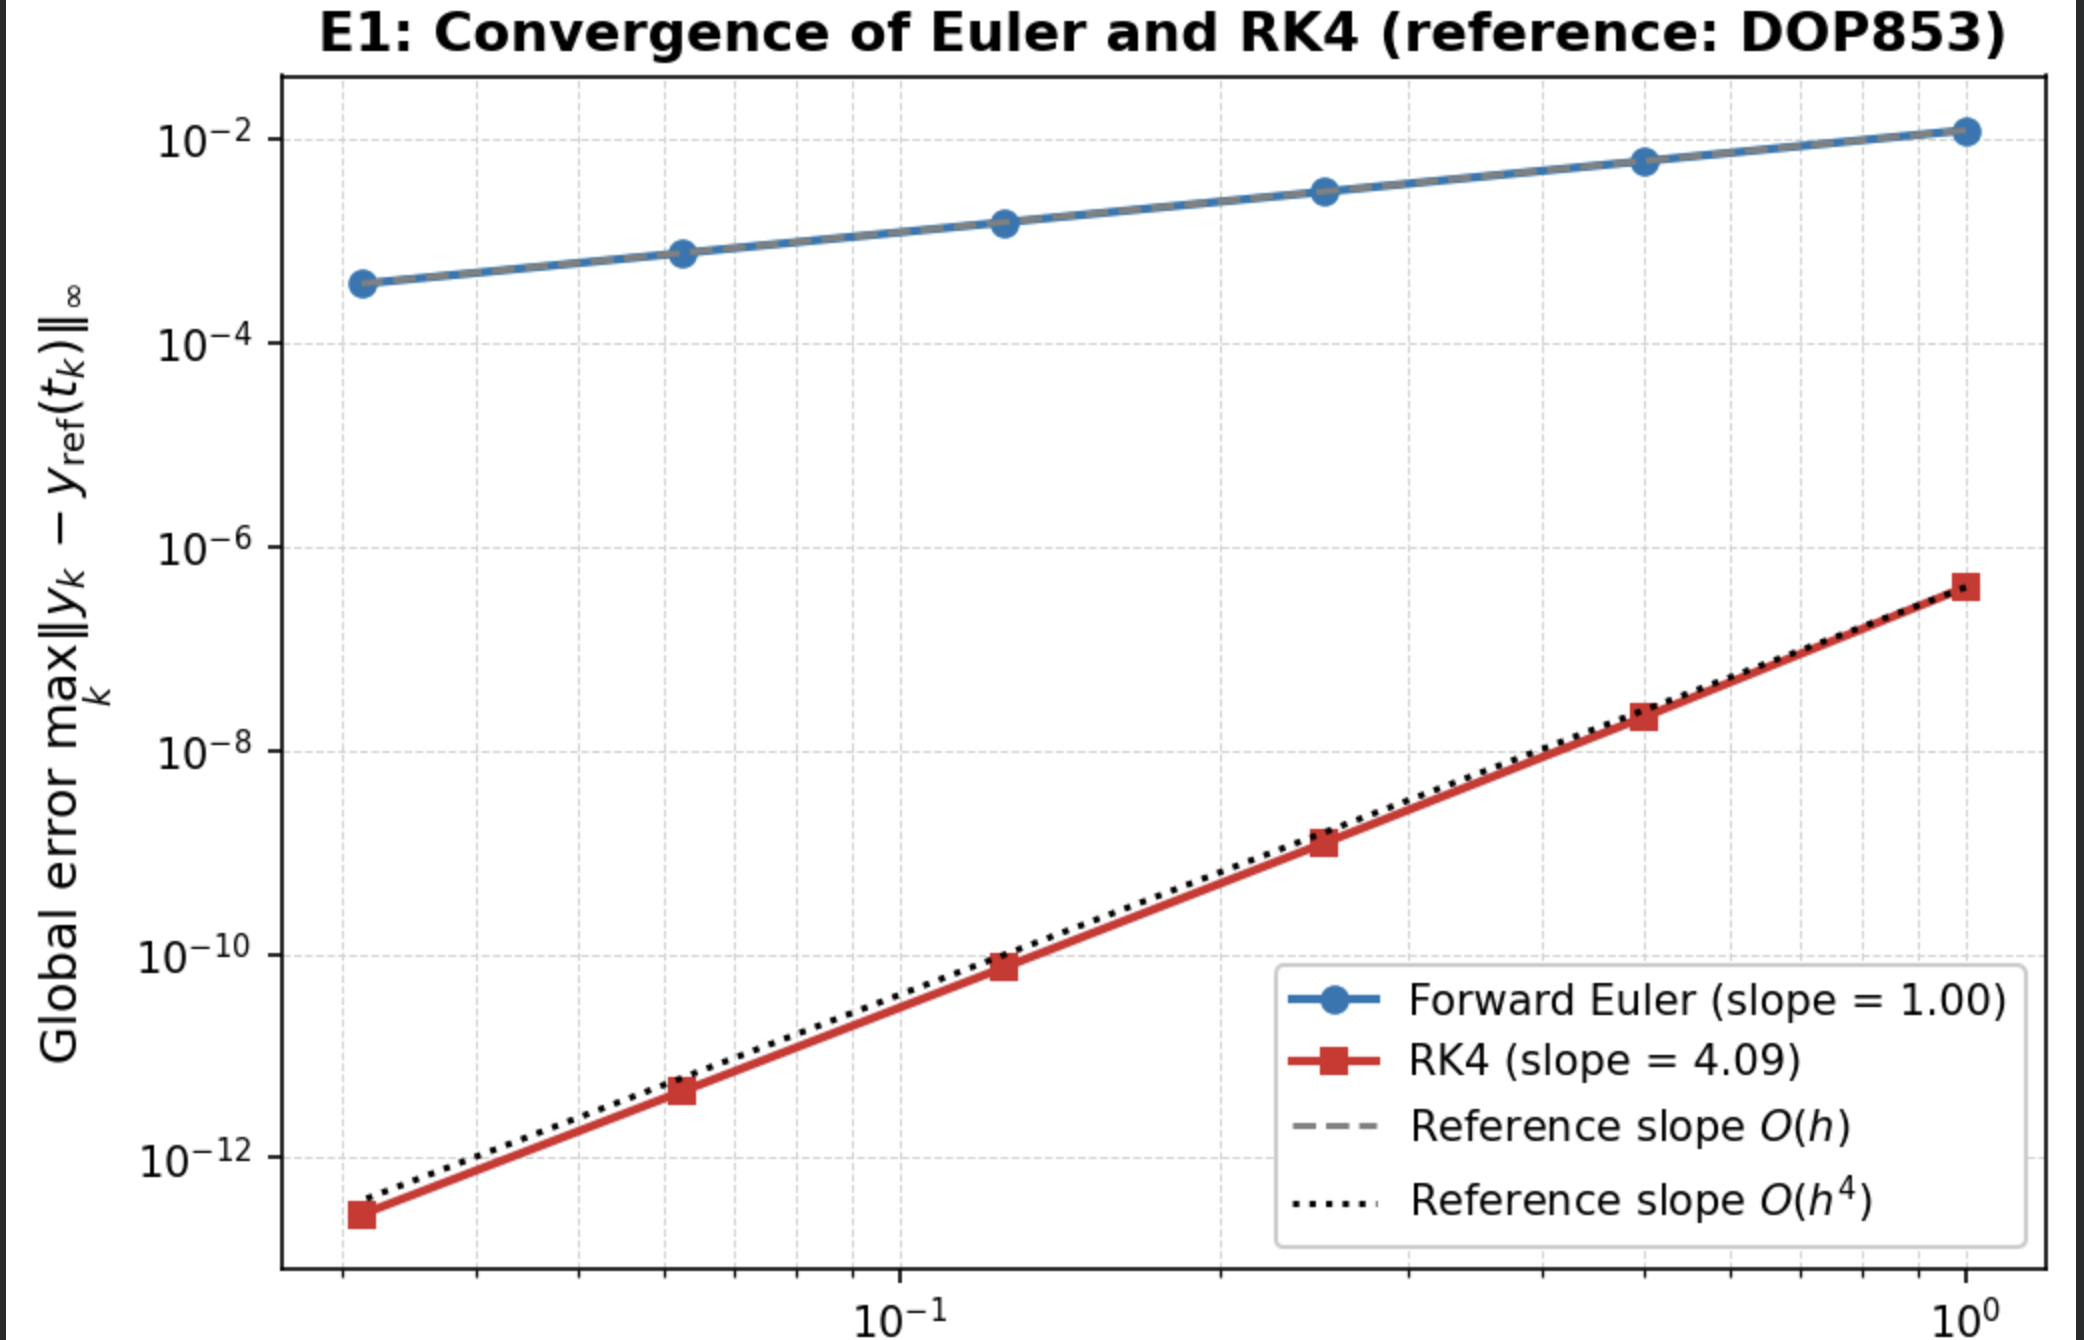
\includegraphics[height=0.50\textheight,trim=10 0 0 0,clip]{figs/fig_e1_convergence.png}\\[1pt]
  {\scriptsize\color{mvMuted} reference lines: slopes 1 and 4}
\column{0.47\textwidth}
  \scriptsize\setlength{\tabcolsep}{3.5pt}
  \begin{tabular}{@{}rcccc@{}}
    \toprule
    $h$ (days) & Euler error & order & RK4 error & order \\
    \midrule
    1       & $1.22\times10^{-2}$ & 1.004 & $4.00\times10^{-7}$  & 4.225 \\
    0.5     & $6.09\times10^{-3}$ & 1.002 & $2.14\times10^{-8}$  & 4.124 \\
    0.25    & $3.04\times10^{-3}$ & 1.001 & $1.23\times10^{-9}$  & 4.061 \\
    0.125   & $1.52\times10^{-3}$ & 1.001 & $7.34\times10^{-11}$ & 4.031 \\
    0.0625  & $7.59\times10^{-4}$ & 1.000 & $4.49\times10^{-12}$ & 4.015 \\
    0.03125 & $3.80\times10^{-4}$ & --    & $2.78\times10^{-13}$ & --    \\
    \midrule
    \multicolumn{2}{@{}l}{fitted slope} & \textbf{1.001} & & \textbf{4.085} \\
    \bottomrule
  \end{tabular}\\[3pt]
  \footnotesize\raggedright
  \begin{itemize}\setlength{\itemsep}{0pt}
    \item Euler: error \textbf{halves} when $h$ halves
    \item RK4: error falls by a factor of about \textbf{16}
    \item RK4's order sits slightly above 4 for large steps and approaches 4 as $h$ shrinks
  \end{itemize}
\end{columns}
\mvTakeaway{\textbf{Result:} observed orders 1.001 and 4.085 match the theory (1 and 4).
At $h=1$ day RK4 is about $3\times10^{4}$ times more accurate than Euler for four times the work per step, so RK4 is used for forward simulation.}
\end{frame}


% ---- Module 4: PINN design, loss, synthetic experiments ----
% ======================================================================
% Module 4: Physics-Informed Neural Networks (PINN) for SEIRD
% Three frames, no title slide: \input this file into the main deck.
%
% Needs in the main preamble:
%   \usepackage{graphicx,booktabs,amssymb,multimedia}
%   \usetikzlibrary{arrows.meta,positioning}
% Figures are in figs/ next to this file. If this file sits in a folder
% (e.g. module4/), add \graphicspath{{module4/}} to the main preamble.
% All numbers are from report/main.tex (final Colab run).
% ======================================================================

% Shared deck colours (same values as Module 1 and Module 5)
\definecolor{mvPINN}{HTML}{7B2D8E}
\definecolor{mvPW}{HTML}{2A9D3A}
\definecolor{mvCB}{HTML}{1F5FBF}
\definecolor{mvInk}{HTML}{1F2933}
\definecolor{mvMuted}{HTML}{5F6B7A}
\definecolor{mvSoft}{HTML}{F3EDF6}
\definecolor{mvRule}{HTML}{C9B6D3}

\providecommand{\mvTakeaway}[1]{%
  \par\vspace{3pt}\noindent
  \fcolorbox{mvRule}{mvSoft}{\parbox{\dimexpr\linewidth-2\fboxsep-2\fboxrule\relax}{\footnotesize\color{mvInk}#1}}}

% -----------------------------------------------------------------------
\begin{frame}{PINN design: architecture and inductive biases}
\framesubtitle{Module 4 \textbullet\ two networks share one physics loss \textbullet\ six design choices enforce SEIRD structure exactly}
\vspace{-2pt}
\begin{columns}[T,onlytextwidth]
\column{0.50\textwidth}
  \footnotesize\raggedright
  \textbf{\color{mvPINN}The observability problem}
  \begin{itemize}\setlength{\itemsep}{1pt}
    \item Surveillance reports two series: cumulative cases $C$ and deaths $D$
    \item Hidden compartments $S,E,I$ are \textbf{never measured}
    \item $\beta(t)$ and $\mu$ must be inferred from $C$ and $D$ alone
  \end{itemize}
  \vspace{3pt}
  \textbf{\color{mvPINN}Observable re-parameterisation}\\[1pt]
  {\small Set $C = I+R+D$ (everything symptomatic). Then $S = N-E-C$ exactly, so mass conservation \emph{cannot be violated} for any network output.\par}
  \vspace{3pt}
  \textbf{\color{mvPINN}Dual-network architecture}
  \begin{itemize}\setlength{\itemsep}{1pt}
    \item \textbf{State net} $g_\theta(\tau)$: $3\times48$ $\tanh$ units, 4 outputs
    \[
      e = e_0\,e^{\tau g_1},\; i = i_0\,e^{\tau g_2},\; c = c_0\,e^{\tau g_3},\; d = d_0+\tau g_4
    \]
    \item \textbf{Transmission net} $h_\phi(\tau)$: $3\times32$ $\tanh$ units,\\ $\beta(\tau)=\operatorname{Softplus}(h_\phi(\tau)+b)>0$
  \end{itemize}
\column{0.47\textwidth}
  \footnotesize\raggedright
  \textbf{\color{mvPINN}Six inductive biases}
  \begin{enumerate}\setlength{\itemsep}{1pt}
    \item \textbf{Hard ICs:} exponential form $e_0 e^{\tau g_1}$ satisfies $e(0)=e_0$ exactly; $\tau$ factor means the gradient of the IC loss is always zero
    \item \textbf{Positivity:} Softplus and exponential forms keep every state $>0$
    \item \textbf{CFR bounds:} $\mu = \gamma\operatorname{CFR}/(1-\operatorname{CFR})$,\; $\operatorname{CFR}\in(0.2,0.8)$, blocks the degenerate $\mu\to 0$ solution
    \item \textbf{Fourier features:} $\sin(k\pi\tau')$ and $\cos(k\pi\tau')$, $k=1,\ldots,4$ overcome spectral bias so $\beta(t)$ changes can be represented inside the window
    \item \textbf{Relative ODE residuals:} each equation divided by its state, so the early (small) phase costs as much as the late (large) phase
    \item \textbf{Smooth prior on $\beta$:} penalty on $(d\beta/d\tau)^2$ makes the inverse problem well-posed
  \end{enumerate}
\end{columns}
\mvTakeaway{\textbf{What the architecture guarantees without training:} $S+E+I+R+D=N$ to machine precision; $e,i,c>0$; initial conditions exact; $\operatorname{CFR}\in(0.2,0.8)$.}
\end{frame}

% -----------------------------------------------------------------------
\begin{frame}{Loss function and training protocol}
\framesubtitle{Module 4 \textbullet\ four terms; Adam brings it close, L-BFGS closes the gap}
\vspace{-2pt}
\begin{columns}[T,onlytextwidth]
\column{0.52\textwidth}
  \footnotesize\raggedright
  \textbf{\color{mvPINN}Total loss}
  \[
    \mathcal{L} = \underbrace{\mathcal{L}_C + \mathcal{L}_D}_{\text{data}} + \mathcal{L}_{\text{ode}} + w_{\text{sm}}\,\mathcal{L}_{\text{smooth}}
  \]
  \vspace{-6pt}
  \begin{align*}
    \mathcal{L}_C &= \tfrac{1}{n_C}\textstyle\sum_k\bigl(c(\tau_k)-C_k/K\bigr)^2 \\
    \mathcal{L}_D &= \tfrac{1}{n_D}\textstyle\sum_k\bigl(d(\tau_k)-D_k/K\bigr)^2 \\
    \mathcal{L}_{\text{ode}} &= \tfrac{1}{N_f}\textstyle\sum_j\Bigl[
      \Bigl(\tfrac{e'-Tf_e}{e}\Bigr)^2\!+\!\Bigl(\tfrac{i'-Tf_i}{i}\Bigr)^2
      \!+\!\cdots\Bigr]_{\!\tau_j} \\
    \mathcal{L}_{\text{smooth}} &= \tfrac{1}{N_f}\textstyle\sum_j\bigl(\tfrac{d\beta}{d\tau}(\tau_j)\bigr)^2
  \end{align*}
  {\scriptsize $K$ = max training case count; $N_f=200$ collocation points; $w_{\text{sm}}=10^{-4}$ (synthetic), $10^{-3}$ (real data); $w_{\text{data}}=w_{\text{ode}}=1$.\par}
  \vspace{3pt}
  \textbf{\color{mvPINN}Why relative ODE residuals?}\\
  {\footnotesize An epidemic grows by orders of magnitude. With plain (absolute) residuals the early phase costs almost nothing. The E6 ablation shows absolute residuals give 75--128\% forward error vs.\ below $2\times10^{-3}$ with relative residuals.\par}
\column{0.45\textwidth}
  \footnotesize\raggedright
  \textbf{\color{mvPINN}Two-stage optimiser}
  \begin{itemize}\setlength{\itemsep}{1pt}
    \item \textbf{Stage 1 -- Adam} (LR $2\times10^{-3}$, cosine decay, 2000 iters): fresh random collocation points each iteration; fast escape from saddle points
    \item \textbf{Stage 2 -- L-BFGS} (strong-Wolfe line search, 2500--6000 iters, fixed linspace grid): second-order convergence to a tight solution
    \item All weights in \textbf{double precision} (float64) for accurate physics residuals
    \item \textbf{Ensemble:} 5 independent seeds; median is the point estimate
  \end{itemize}
  \vspace{4pt}
  \textbf{\color{mvPINN}Forecasting}\\
  {\footnotesize Hold $\beta$ at its mean over the last 14 training days; keep learned $\mu$; integrate forward with DOP853. Forecast is the median over seeds. The assumption that $\beta$ stays constant limits predictive horizon.\par}
  \vspace{4pt}
  \textbf{\color{mvMuted}E6 ablation headline}\\
  {\footnotesize Adam-only: $e(t)$ error $96\%$; $w_{\text{ode}}=10$: errors triple; no Fourier features: $\beta$ RMSE $+38\%$.}
\end{columns}
\end{frame}

% -----------------------------------------------------------------------
\begin{frame}{Synthetic experiments: E2 forward, E3 inverse $\beta(t)$, E4 hidden states}
\framesubtitle{Module 4 \textbullet\ no real data; ground truth is known; PINN is tested against DOP853}
\vspace{-4pt}
\begin{columns}[T,onlytextwidth]
\column{0.50\textwidth}
  \centering
  \includegraphics[height=0.28\textheight]{figs/fig_e2_forward_pinn.png}\\
  {\scriptsize\color{mvMuted} E2: forward PINN (markers) vs.\ DOP853 (lines) and pointwise error}\\[4pt]
  \scriptsize\setlength{\tabcolsep}{3pt}
  \begin{tabular}{@{}lcc@{}}
    \toprule
    Quantity & 1\% noise & 5\% noise \\
    \midrule
    $\beta(t)$ rel.\ $L_2$ & $11.0\%\pm0.7\%$ & $11.6\%\pm0.6\%$ \\
    $\mu$ rel.\ error       & $4.6\%\pm0.3\%$  & $5.4\%\pm1.0\%$  \\
    hidden $s(t)$           & $0.36\%\pm0.03\%$ & $0.46\%\pm0.09\%$ \\
    hidden $e(t)$           & $5.8\%\pm0.6\%$   & $6.4\%\pm0.7\%$  \\
    hidden $i(t)$           & $5.8\%\pm0.4\%$   & $6.5\%\pm0.8\%$  \\
    \bottomrule
  \end{tabular}\\[1pt]
  {\tiny\color{mvMuted} E3/E4: mean $\pm$ SD over 5 seeds; $\beta$ drops 0.55$\to$0.25 at day 30}
\column{0.48\textwidth}
  \centering
  \includegraphics[width=\linewidth,height=0.28\textheight,keepaspectratio]{figs/fig_e3_inverse_beta.png}\\
  {\scriptsize\color{mvMuted} E3: recovered $\beta(t)$ (band = seed range, 5\% noise)}\\[2pt]
  \includegraphics[width=\linewidth,height=0.28\textheight,keepaspectratio]{figs/fig_e4_hidden_states.png}\\
  {\scriptsize\color{mvMuted} E4: reconstructed $s(t)$, $e(t)$, $i(t)$ from cases and deaths only}
\end{columns}
\vspace{1pt}
\mvTakeaway{\textbf{E2:} worst compartment $< 2\times10^{-3}$; conservation $2\times10^{-16}$ (machine zero).
\textbf{E3:} a sharp $\beta$ change recovered within 11\%; $5\times$ more noise costs $<1$ pp.
\textbf{E4:} susceptible fraction recovered within $0.5\%$ from \emph{zero} direct measurements.}
\end{frame}


% ---- Module 5: real data, rolling forecasts, what the PINN adds ----
% ======================================================================
% Module 5: real-data results (E5 held-out forecast, E7 rolling forecasts)
% Three frames, no title slide: \input this file into the main deck.
%
% Needs in the main preamble:  \usepackage{graphicx,booktabs,amssymb}
% Figures are in figs/ next to this file. If this file sits in a folder
% (e.g. module5/), add \graphicspath{{module5/}} to the main preamble.
% All numbers are from report/main.tex (final Colab run, WHO data).
% ======================================================================

% Method colours match the figures (pinn_figures.py, METHOD_STYLE)
\definecolor{mvPINN}{HTML}{7B2D8E}
\definecolor{mvPW}{HTML}{2A9D3A}
\definecolor{mvCB}{HTML}{1F5FBF}
\definecolor{mvInk}{HTML}{1F2933}
\definecolor{mvMuted}{HTML}{5F6B7A}
\definecolor{mvSoft}{HTML}{F3EDF6}
\definecolor{mvRule}{HTML}{C9B6D3}

\providecommand{\mvPINN}{\textcolor{mvPINN}{\textbf{PINN}}}
\providecommand{\mvPW}{\textcolor{mvPW}{\textbf{Piecewise-$\beta$}}}
\providecommand{\mvCB}{\textcolor{mvCB}{\textbf{Constant-$\beta$}}}
\providecommand{\mvTakeaway}[1]{%
  \par\vspace{3pt}\noindent
  \fcolorbox{mvRule}{mvSoft}{\parbox{\dimexpr\linewidth-2\fboxsep-2\fboxrule\relax}{\footnotesize\color{mvInk}#1}}}

% ----------------------------------------------------------------------
\begin{frame}{E5: Held-out forecast on WHO data}
\framesubtitle{Module 5 \textbullet\ WHO lab-confirmed reports, Sierra Leone\\ fit: 29 Aug 2014 -- 24 Feb 2015 \textbullet\ test: 25 Feb -- 25 Apr 2015, never seen}
\vspace{-2pt}
\begin{columns}[T,onlytextwidth]
\column{0.495\textwidth}
  \centering
  \includegraphics[height=0.54\textheight]{figs/e5_cases.png}\\[1pt]
  \scriptsize
  \begin{tabular}{@{}lccc@{}}
    \toprule
    Cases, relative error & \mvPINN & \mvPW & \mvCB \\
    \midrule
    60-day forecast & 1.35\% & \textbf{0.82\%} & 28.6\% \\
    \bottomrule
  \end{tabular}
\column{0.495\textwidth}
  \centering
  \includegraphics[height=0.54\textheight]{figs/e5_deaths.png}\\[1pt]
  \scriptsize
  \begin{tabular}{@{}lccc@{}}
    \toprule
    Deaths, relative error & \mvPINN & \mvPW & \mvCB \\
    \midrule
    60-day forecast & 11.8\% & 12.9\% & \textbf{10.7\%} \\
    \bottomrule
  \end{tabular}
\end{columns}
\mvTakeaway{\textbf{A time-varying $\beta$ is what matters:} \mvCB\ keeps growing and misses cases by 29\%.
\mvPINN\ is a close second to \mvPW\ on cases (single seeds: 0.28--1.75\%).
\textbf{Deaths defeat every method} (11--13\%): WHO added 463 deaths but only 361 cases in the test window.}
\end{frame}

% ----------------------------------------------------------------------
\begin{frame}{E7: Rolling 4-week forecasts across the epidemic}
\framesubtitle{Module 5 \textbullet\ 8 origins, every 28 days from 16 Jan to 31 Jul 2015 \textbullet\ each fit sees only the previous 8 weeks}
\vspace{-4pt}
\centering
\includegraphics[height=0.52\textheight]{figs/e7_rolling.png}\\[3pt]
\begin{columns}[T,onlytextwidth]
\column{0.50\textwidth}
  \scriptsize\setlength{\tabcolsep}{4pt}
  \begin{tabular}{@{}lccc@{}}
    \toprule
    Mean of 8 origins & Cases MAE & New cases, 4 wk & Deaths MAE \\
    \midrule
    \mvPINN\ (3 seeds) & \textbf{96.8}  & \textbf{148.2} & 69.7 \\
    \mvPW              & 106.5          & 167.8          & \textbf{42.0} \\
    \mvCB              & 120.9          & 192.5          & 50.7 \\
    \bottomrule
  \end{tabular}\\[1pt]
  {\tiny\color{mvMuted} Errors in people. ``New cases, 4 wk'': error in new cases over the horizon.}
\column{0.46\textwidth}
  \footnotesize
  \begin{itemize}\setlength{\itemsep}{1pt}
    \item[$\checkmark$] \textbf{Cases:} \mvPINN\ is best on average, 20\% below \mvCB, and beats \mvPW\ at 6 of 8 origins.
    \item[$\times$] \textbf{Deaths:} \mvPINN\ is worst; its death forecast inherits any error in the learned $\mu$.
  \end{itemize}
\end{columns}
\end{frame}

% ----------------------------------------------------------------------
\begin{frame}{What the PINN adds, and what it costs}
\framesubtitle{Module 5 \textbullet\ interpretation and limitations}
\vspace{-2pt}
\begin{columns}[T,onlytextwidth]
\column{0.47\textwidth}
  \centering
  \includegraphics[height=0.49\textheight]{figs/e5_rt.png}\\[1pt]
  \scriptsize\raggedright
  \textbf{Learned $R_t = \beta(t)\,s(t)/(\gamma+\mu)$}, E5 training window (5 seeds, median bold):
  \begin{itemize}\setlength{\itemsep}{0pt}
    \item peak $\approx 1.28$ in early Oct 2014
    \item crosses 1 in mid-Nov 2014: the epidemic turns
    \item $\approx 0.6$ in mid-Jan 2015, $\approx 0.8$ by late Feb 2015
  \end{itemize}
\column{0.50\textwidth}
  \footnotesize\raggedright
  \textbf{\color{mvPINN}What it gives that least squares does not}
  \begin{itemize}\setlength{\itemsep}{1pt}
    \item a continuous $R_t(t)$ with no breakpoints to choose
    \item the case-fatality ratio, learned: 0.347--0.357 across seeds
    \item the hidden compartments $S, E, I$ alongside the fit
  \end{itemize}
  \vspace{2pt}
  \textbf{\color{mvMuted}What it costs}
  \begin{itemize}\setlength{\itemsep}{1pt}
    \item 1--2 min per fit (Colab CPU) vs.\ seconds for least squares
    \item needs a seed ensemble: single seeds vary (0.28--1.75\%)
    \item forecasts hold $\beta$ at its recent value, so they cannot foresee a new intervention or a resurgence
  \end{itemize}
\end{columns}
\mvTakeaway{\textbf{Honest verdict:} on cases the PINN forecasts about as well as the best classical fit; on deaths it does worse.
Its real value is an interpretable, continuous picture of transmission.}
\end{frame}


\end{document}
